%==============================================================================
% T.Y. B.Tech. Project Presentation — COEP Tech format (Beamer)
% UWB Indoor RTLS + Live 3D Digital Twin
% Compile with pdflatex (e.g. on Overleaf). Needs: beamer, graphicx.
% Images expected next to this file: COEP_Tech_University_Logo.jpg, twin_screenshot.png,
%                                    architecture.png, accuracy_chart.png, uml_class.png
%==============================================================================
\documentclass[aspectratio=169,10pt]{beamer}

% --- Theme: reproduce the uploaded COEP format -------------------------------
\usetheme{Frankfurt}                       % miniframes header (section names + dots)
\usecolortheme{default}                    % beamer blue
\useinnertheme[shadow=true]{rounded}       % rounded title block with drop shadow
\setbeamertemplate{navigation symbols}{}   % no nav symbols

\usepackage{graphicx}
\usepackage{booktabs}
\usepackage{amsmath}

% ◀ triangle bullets (as in the uploaded format)
\setbeamertemplate{itemize item}{\small\raise0.4pt\hbox{$\blacktriangleleft$}}
\setbeamertemplate{itemize subitem}{\footnotesize\raise0.4pt\hbox{$\blacktriangleleft$}}
\setbeamertemplate{itemize subsubitem}{\footnotesize\raise0.4pt\hbox{$\blacktriangleleft$}}

% Custom footline: logo (left) | institute (centre) | frame number (right)
\setbeamertemplate{footline}{%
  \leavevmode%
  \hbox{%
  \begin{beamercolorbox}[wd=.15\paperwidth,ht=4.5ex,dp=1.6ex,left]{}%
    \hspace{4pt}\raisebox{-1ex}{
\includegraphics[height=4.5ex]{COEP_Tech_University_Logo.jpg}}%
  \end{beamercolorbox}%
  \begin{beamercolorbox}[wd=.70\paperwidth,ht=4.5ex,dp=1.6ex,center]{}%
    {\color{structure}\small COEP Technological University [COEP Tech]}\\[1pt]%
    {\color{structure}\tiny (A Unitary Public University of Government of Maharashtra)}%
  \end{beamercolorbox}%
  \begin{beamercolorbox}[wd=.15\paperwidth,ht=4.5ex,dp=1.6ex,right]{}%
    \usebeamerfont{page number in head/foot}%
    \insertframenumber{} / \inserttotalframenumber\hspace{6pt}%
  \end{beamercolorbox}}%
  \vskip0pt%
}

% --- Title metadata ----------------------------------------------------------
\title[UWB Indoor RTLS + Digital Twin]{UWB Indoor Real-Time Location System with a Live 3D Digital Twin}
\subtitle{B. Tech. Project — Computer Science \& Engineering}
\author[Kale, Lohiya, Vasaikar]{Nahush Kale \and Akshad Lohiya \and Purnank Vasaikar}
\institute[COEP Tech]{Department of Computer Science \& Engineering\\
COEP Technological University, Pune\\[4pt]
\textit{Under the guidance of} Prof. Dr. H. D. Gadade}
\date{September 22, 2026}
\titlegraphic{
\includegraphics[height=1.6cm]{COEP_Tech_University_Logo.jpg}}

\begin{document}

% --- Title slide -------------------------------------------------------------
{\setbeamertemplate{footline}{}          % clean title slide (institute shown by title)
\begin{frame}[plain]
  \titlepage
\end{frame}}

% --- Outline -----------------------------------------------------------------
\begin{frame}{Outline}
  \tableofcontents
\end{frame}

%==============================================================================
\section{Introduction}
%==============================================================================
\begin{frame}{Introduction}
  \begin{itemize}
    \item \textbf{UWB (Ultra-Wideband):} radio that sends very short, very wide-band
          pulses $\Rightarrow$ fine time resolution and strong multipath rejection
          $\Rightarrow$ \textbf{centimetre-to-decimetre} ranging indoors.
    \item \textbf{RTLS (Real-Time Location System):} track tagged assets and people
          \emph{live}, indoors, where GPS cannot reach.
    \item \textbf{Digital Twin:} a live, labelled 3D model of the physical floor that
          shows every tracked item moving in real time.
    \item \textbf{Our system:} ceiling-mounted UWB anchors range the tags via
          \textbf{DS-TWR}, a position engine turns those ranges into a smooth track,
          and a browser dashboard renders the room, anchors and tags.
  \end{itemize}
\end{frame}

\begin{frame}{Why UWB Indoors}
  \begin{itemize}
    \item GPS is \textbf{blocked} indoors; Wi-Fi / BLE give \textbf{metre-to-tens-of-metre}
          error (narrowband, multipath-prone).
    \item UWB is the leading technology for high-accuracy indoor positioning.
    \item \textbf{Target application:} warehouse-scale asset \& personnel tracking ---
          inventory location, worker safety, geofencing / zone alerts.
    \item \textbf{Hardware:} Makerfabs \textbf{MaUWB\_DW3000} nodes; firmware performs
          \textbf{DS-TWR ranging} and reports a distance per anchor plus signal-power
          diagnostics.
  \end{itemize}
\end{frame}

%==============================================================================
\section{Literature Review}
%==============================================================================
\begin{frame}{Literature Review}
  \begin{columns}[T]
    \begin{column}{0.52\textwidth}
      $1^{st}$ column --- \textbf{Key studies}
      \begin{itemize}\small
        \item Paszek et al., \emph{Sensors} 2021 --- UWB LOS/NLOS \textbf{simulator} + accuracy analysis.
        \item \emph{Appl. Sci.} 2025 --- \textbf{NLOS-exclusion} positioning (RMSE 0.124~m, $\approx$24\% $\uparrow$).
        \item \emph{Appl. Sci.} 2024 --- UWB RTLS deployment \& error study.
        \item Zhao et al., IJRR 2024 --- \textbf{UTIL} dataset: raw TDOA + power-diff + mm Vicon truth.
        \item \emph{Alexandria Eng. J.} 2018 --- UWB error modelling.
      \end{itemize}
    \end{column}
    \begin{column}{0.48\textwidth}
      $2^{nd}$ column --- \textbf{Takeaways}
      \begin{itemize}\small
        \item NLOS-aware \textbf{weighting} is the single biggest accuracy lever.
        \item A \textbf{hardware-faithful simulator} lets the full pipeline be built before hardware arrives.
        \item Real \textbf{mm-ground-truth} data (UTIL) enables noise/NLOS \textbf{calibration} and EKF validation.
        \item \textbf{DS-TWR} cancels device clock drift $\Rightarrow$ \emph{no} anchor time-synchronisation needed.
      \end{itemize}
    \end{column}
  \end{columns}
\end{frame}

\begin{frame}{Reference Dataset: UTIL}
  \begin{itemize}
    \item UofT UTIAS DSL, IJRR 2024 --- Decawave \textbf{DWM1000}; 4 anchor
          constellations, $\approx$150~min of flights.
    \item Provides raw UWB \textbf{TDOA}, \textbf{SNR / power-difference} (LOS/NLOS labels),
          IMU, altitude, \textbf{mm-accurate Vicon ground truth}, plus a reference EKF and parsers.
    \item \textbf{Cross-radio caveat:} DWM1000 $\neq$ our DW3000 $\Rightarrow$ a fitted model is a
          \emph{prior needing DW3000 recalibration}, not a direct transplant.
  \end{itemize}
\end{frame}

%==============================================================================
\section{Research Gap}
%==============================================================================
\begin{frame}{Research Gap}
  \begin{itemize}
    \item Many indoor-positioning demos \textbf{shortcut}: they display measured ranges but stream the
          \emph{true} position to the UI $\Rightarrow$ no real solve, no NLOS handling, \textbf{fake accuracy}.
    \item NLOS down-weighting is usually \textbf{hand-tuned constants}, not fitted to real error data.
    \item Simulator and hardware are typically \textbf{separate codebases} $\Rightarrow$ costly, error-prone
          hardware integration.
    \item Weak \textbf{height (z) observability} with co-planar ceiling anchors is rarely addressed.
  \end{itemize}
  \vspace{4pt}
  \textbf{Our gap-closing contributions:}
  \begin{itemize}
    \item A pipeline that \textbf{actually estimates} position from noisy, partly-NLOS ranges.
    \item A \textbf{data-driven} NLOS/noise model fitted on real mm-truth UWB data.
    \item \textbf{One codebase} --- simulator $\leftrightarrow$ hardware behind a single interface.
  \end{itemize}
\end{frame}

%==============================================================================
\section{Problem Statement}
%==============================================================================
\begin{frame}{Problem Statement}
  \begin{block}{Goal}
    Build an \textbf{end-to-end indoor RTLS} that ranges tags from ceiling anchors,
    \alert{solves} each tag's position from noisy / partly-NLOS ranges, \alert{smooths}
    the estimate over time, and \alert{visualises} it live on a 3D digital twin.
  \end{block}
  \begin{itemize}
    \item The estimate must be \emph{honest}: position is \textbf{computed} from measurements,
          not read from ground truth --- and its accuracy is reported against truth.
    \item Architected so the \emph{same software} runs against a realistic simulator today
          and real UWB hardware tomorrow.
    \item Hardware integration confined to a \textbf{single drop-in source file}
          (\texttt{SimAnchorSource} $\rightarrow$ \texttt{HardwareAnchorSource}).
  \end{itemize}
\end{frame}

\begin{frame}{Objectives}
  \begin{enumerate}
    \item Define a single versioned \textbf{data contract} shared by simulator \& hardware.
    \item Build a hardware-faithful \textbf{DS-TWR simulator} (LOS/NLOS, antenna-delay bias,
          power diagnostics, dropped readings).
    \item Implement a \textbf{multilateration solver} with NLOS down-weighting from the DW3000 power gap.
    \item Fuse fixes with a \textbf{constant-velocity Kalman filter}
          $\Rightarrow$ smooth track + velocity + uncertainty.
    \item Render a config-driven \textbf{3D digital twin} (trails, uncertainty rings,
          zones, live accuracy HUD).
    \item \textbf{Calibrate \& validate} the noise / NLOS model on real mm-truth UWB data (UTIL).
    \item Keep hardware integration to a \textbf{single file}.
  \end{enumerate}
\end{frame}

%==============================================================================
\section{Key Concepts}
%==============================================================================
\begin{frame}{Key Concepts (1/4) --- UWB Positioning Basics}
  \begin{block}{UWB --- Ultra-Wideband}
    Radio using very short pulses over a very wide bandwidth ($>$500~MHz) $\Rightarrow$
    fine time resolution + strong multipath rejection $\Rightarrow$ centimetre-level ranging.
  \end{block}
  \begin{columns}[T]
    \begin{column}{0.5\textwidth}
      \begin{itemize}\small
        \item \textbf{RTLS:} Real-Time Location System --- live indoor tracking of tagged items.
        \item \textbf{Anchor:} fixed node of \emph{known} coordinates (ceiling-mounted).
        \item \textbf{Tag:} mobile node on the tracked asset / person.
      \end{itemize}
    \end{column}
    \begin{column}{0.5\textwidth}
      \begin{itemize}\small
        \item \textbf{LOS:} Line-of-Sight --- clear direct path; small error.
        \item \textbf{NLOS:} Non-Line-of-Sight --- path blocked; signal reflects, so the range reads
              \alert{longer} --- a positive \emph{bias}, not just noise.
      \end{itemize}
    \end{column}
  \end{columns}
\end{frame}

\begin{frame}{Key Concepts (2/4) --- Ranging \& Observation Models}
  \begin{block}{TWR / DS-TWR --- (Double-Sided) Two-Way Ranging}
    Anchor and tag exchange timed messages to measure a \textbf{distance}. \emph{Double-sided}
    adds a message so device clock-drift cancels $\Rightarrow$ \alert{no anchor time-sync needed}.
    This is exactly what our DW3000 hardware reports.
  \end{block}
  \begin{columns}[T]
    \begin{column}{0.5\textwidth}
      \begin{itemize}\small
        \item \textbf{TOA:} Time-of-Arrival --- absolute travel time $\to$ a range.
        \item \textbf{TDOA:} Time-Difference-of-Arrival --- \emph{synchronised} anchors compare
              arrival times; each anchor pair $\to$ a hyperbola.
      \end{itemize}
    \end{column}
    \begin{column}{0.5\textwidth}
      \begin{block}{Range vs TDOA}
        \footnotesize Range needs no sync but a direct distance; TDOA scales to many tags but needs
        tightly synced anchors. Our pipeline is \textbf{range-based}; a walled-off module handles TDOA.
      \end{block}
    \end{column}
  \end{columns}
\end{frame}

\begin{frame}{Key Concepts (3/4) --- Position Solving}
  \begin{block}{Multilateration / Trilateration}
    Recover a tag's position from $\geq 3$ anchor ranges by intersecting range circles / spheres ---
    solved as a least-squares fit when the measurements are noisy.
  \end{block}
  \begin{itemize}\small
    \item \textbf{WLS --- Weighted Least Squares:} each anchor's residual is weighted by its
          trustworthiness, so unreliable links influence the solution less.
    \item \textbf{Power diagnostics:} DW3000 reports \textbf{received power} (\texttt{rxPower}) and
          \textbf{first-path power} (\texttt{fpPower}); a large \texttt{rxPower$-$fpPower} gap $\Rightarrow$
          an attenuated first path $\Rightarrow$ likely \alert{NLOS}.
    \item \textbf{NLOS down-weighting:} that power gap sets the WLS weight, so a biased (long) NLOS
          range cannot drag the fix.
  \end{itemize}
\end{frame}

\begin{frame}{Key Concepts (4/4) --- State Estimation \& Visualisation}
  \begin{columns}[T]
    \begin{column}{0.52\textwidth}
      \begin{block}{Kalman Filter (KF)}
        \footnotesize A recursive \emph{predict $\to$ update} estimator that fuses a motion model with
        noisy measurements to output a smoothed state and its \textbf{covariance} (uncertainty).
      \end{block}
      \begin{itemize}\small
        \item \textbf{CV model:} constant-velocity motion, state $[x,z,v_x,v_z]$.
        \item \textbf{EKF --- Extended KF:} a KF for \emph{nonlinear} measurements (e.g.\ TDOA),
              linearised at each step.
      \end{itemize}
    \end{column}
    \begin{column}{0.48\textwidth}
      \begin{block}{Digital Twin}
        \footnotesize A live, labelled 3D model of the physical floor rendering every tracked tag,
        its uncertainty ellipse, trail and zone in real time.
      \end{block}
      \begin{itemize}\small
        \item \textbf{Covariance / uncertainty ellipse:} how sure the filter is of a position.
        \item \textbf{Ground truth:} a reference (mm Vicon truth in UTIL) to measure error against.
      \end{itemize}
    \end{column}
  \end{columns}
\end{frame}

%==============================================================================
\section{Work Done}
%==============================================================================
\begin{frame}{Work Done --- System Architecture}
  \begin{center}
    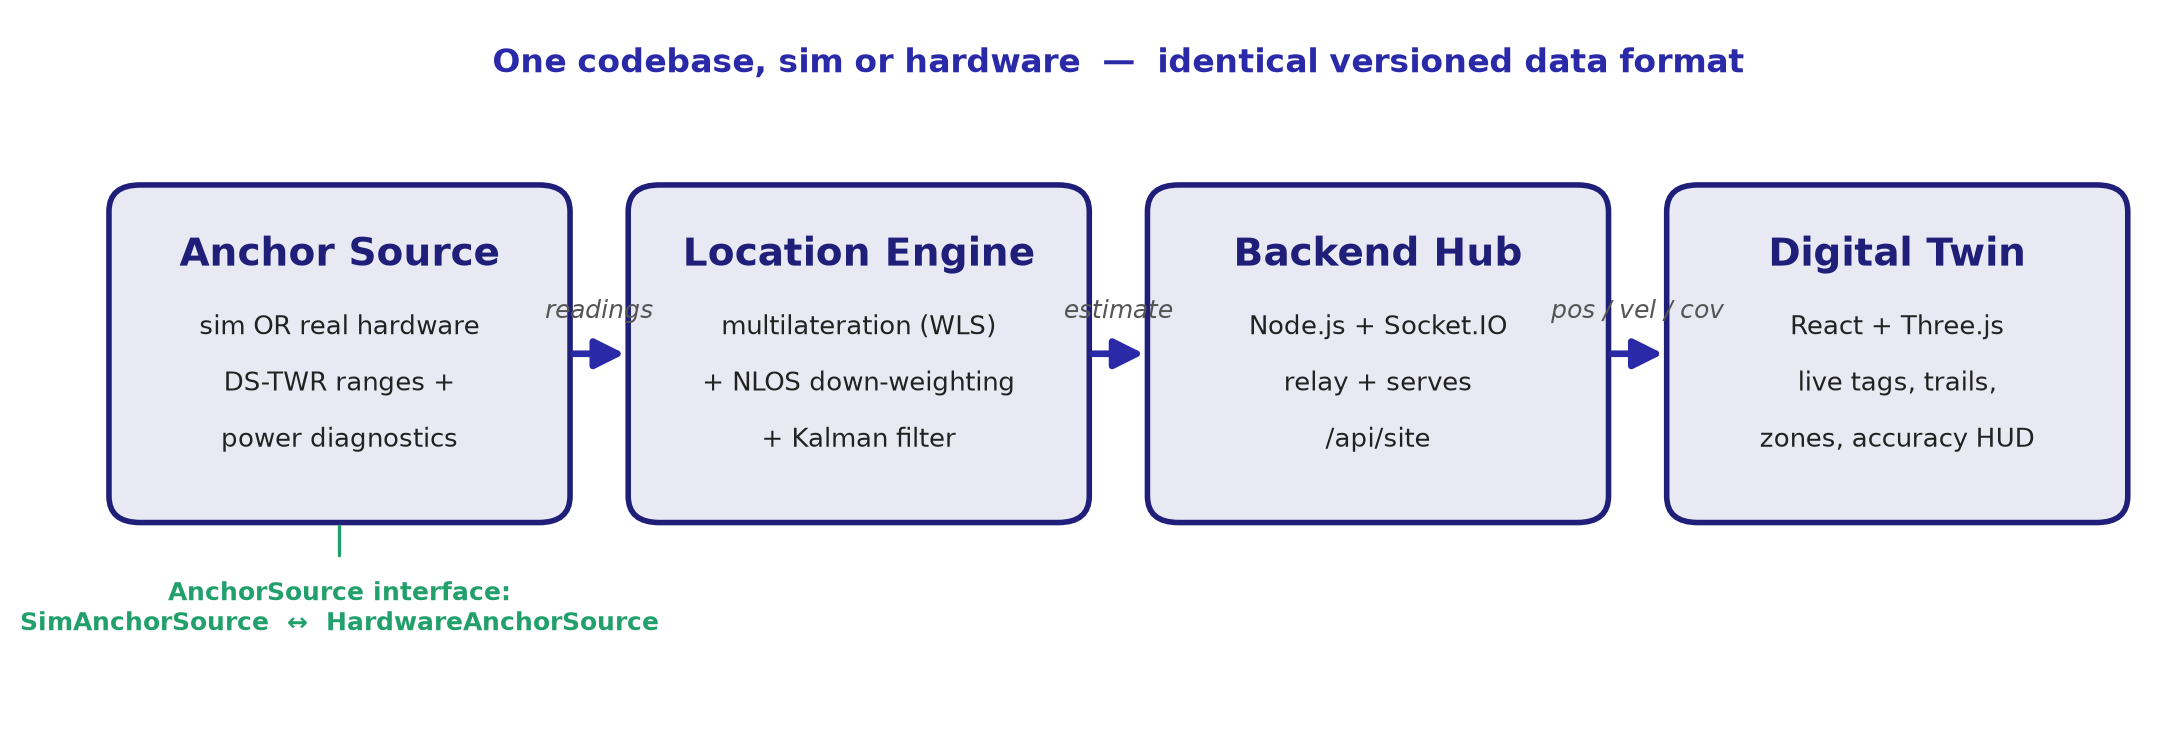
\includegraphics[width=0.92\textwidth]{architecture.png}
  \end{center}
  \vspace{-2pt}
  \begin{itemize}\small
    \item \textbf{Anchor Source} emits per-anchor \emph{range + power diagnostics};
          \textbf{Location Engine} solves + filters; \textbf{Backend} relays + serves \texttt{/api/site};
          \textbf{Frontend} visualises the \emph{estimated} state.
    \item \textbf{Shared site config} (\texttt{site.json}, metres): anchors, walls+material, zones, tag routes,
          ranging/noise model --- every value \textbf{provenance-tagged}.
  \end{itemize}
\end{frame}

\begin{frame}{Work Done --- UML Class Diagram}
  \begin{center}
    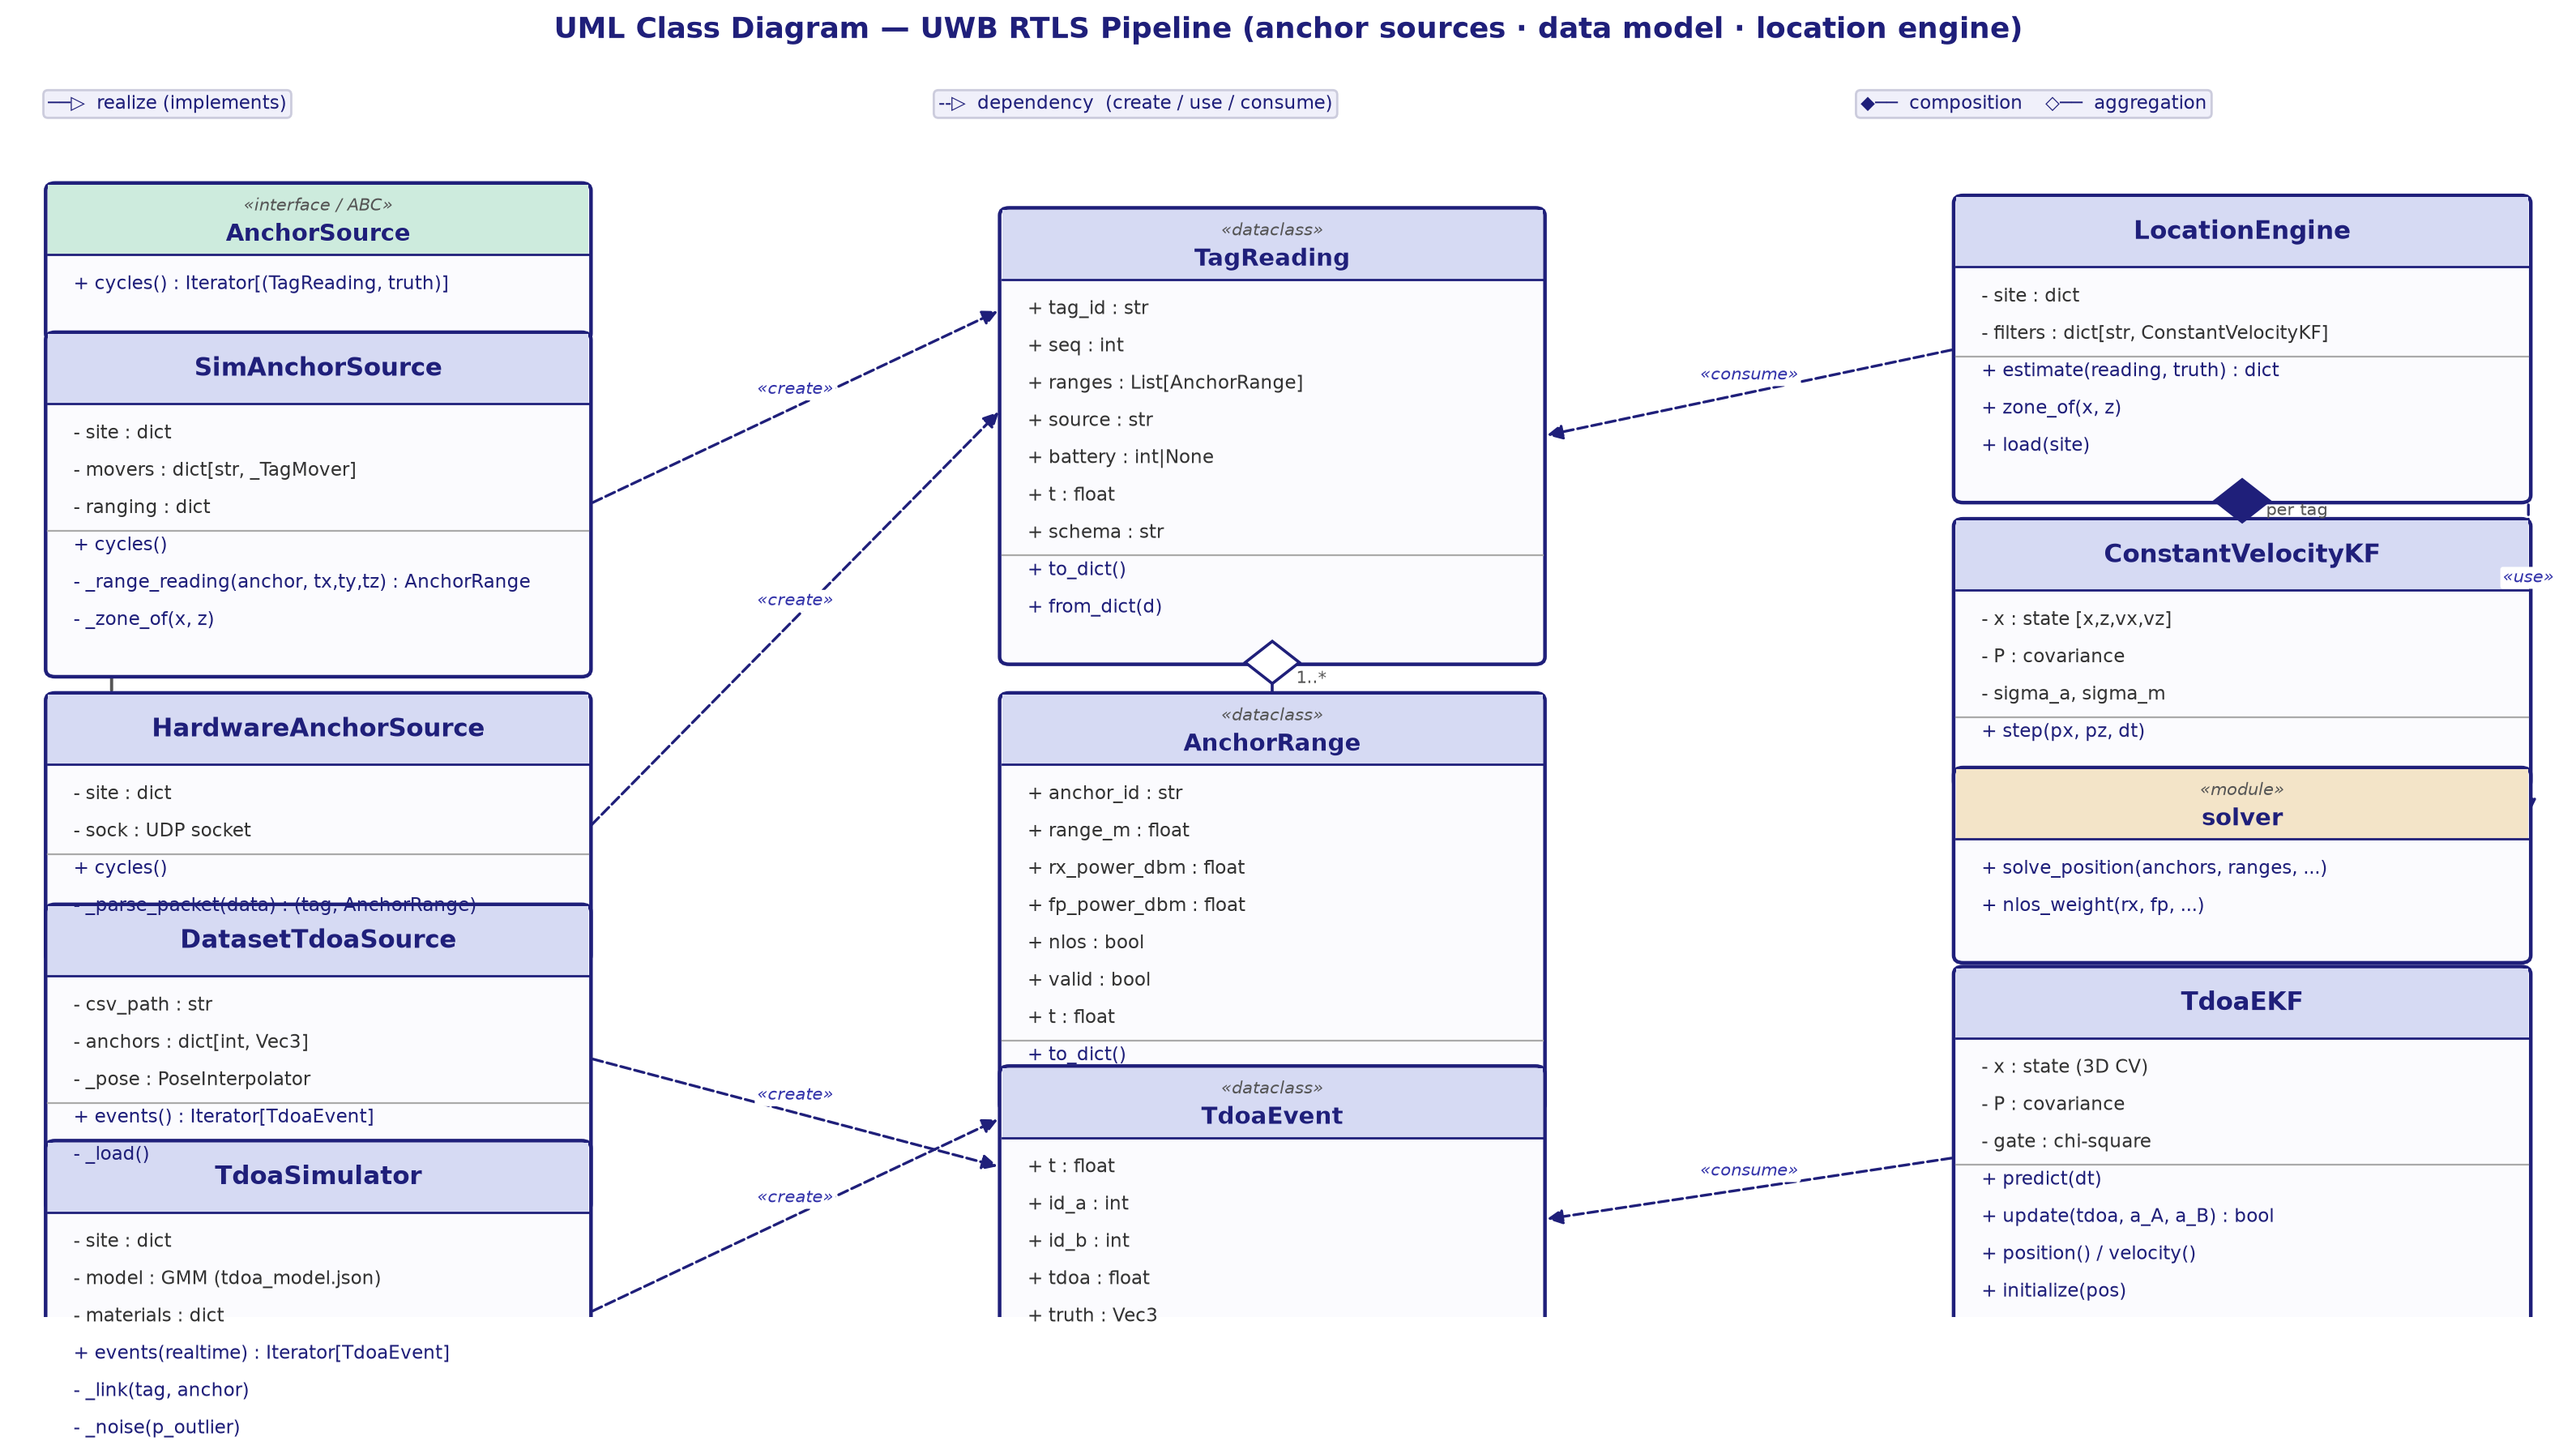
\includegraphics[height=0.83\textheight]{uml_class.png}
  \end{center}
\end{frame}

\begin{frame}{Work Done --- Data Contracts}
  One versioned schema is what makes simulator and hardware interchangeable.
  \begin{columns}[T]
    \begin{column}{0.5\textwidth}
      \begin{block}{Reading (source $\rightarrow$ engine) --- \texttt{uwb.reading/1}}
        \footnotesize Per anchor:
        \begin{itemize}\scriptsize
          \item \texttt{range} --- already contains bias + noise + any NLOS excess
          \item \texttt{rxPower}, \texttt{fpPower} --- the NLOS diagnostic
          \item \texttt{nlos}, \texttt{valid}, timestamp
        \end{itemize}
        \alert{No ground truth reaches the solver.}
      \end{block}
    \end{column}
    \begin{column}{0.5\textwidth}
      \begin{block}{Estimate (engine $\rightarrow$ twin)}
        \footnotesize Per tag:
        \begin{itemize}\scriptsize
          \item \texttt{pos}, \texttt{vel}, \texttt{cov} --- filtered state + uncertainty
          \item \texttt{raw} --- pre-Kalman fix, for comparison
          \item \texttt{truth} --- sim only, drives the accuracy HUD
          \item \texttt{zone}, \texttt{alerts}
        \end{itemize}
      \end{block}
    \end{column}
  \end{columns}
\end{frame}

\begin{frame}{Work Done --- Site Config \& Mapping Platform}
  \begin{columns}[T]
    \begin{column}{0.52\textwidth}
      \begin{block}{\texttt{site.json} --- single source of truth (metres)}
        \footnotesize Anchors, walls (+material), labelled zones, tag routes, and the
        ranging / noise + Kalman model. Every value carries a \textbf{provenance} tag
        (guessed / measured / tested / calibrated).
      \end{block}
      \begin{itemize}\small
        \item Read by \emph{both} the simulator and the twin --- one edit updates the whole system.
        \item Coordinates in \textbf{local metres}, not GPS lat/lon.
      \end{itemize}
    \end{column}
    \begin{column}{0.48\textwidth}
      \begin{block}{Mapping platform (Mappedin-style)}
        \footnotesize
        \begin{itemize}\small
          \item \textbf{Map library:} create / list / delete maps, each with an unguessable share key.
          \item \textbf{2D editor:} draw walls / zones, place anchors, lay out routes.
          \item \textbf{Save \& Apply} hot-reloads sim, solver \& 3D twin --- no restart.
        \end{itemize}
      \end{block}
    \end{column}
  \end{columns}
  \vspace{2pt}
  \begin{center}\footnotesize
  \textbf{Stack:}~ Python (NumPy / SciPy) ~$\cdot$~ Node.js + Socket.IO ~$\cdot$~ React + Three.js ~$\cdot$~ pytest
  \end{center}
\end{frame}

\begin{frame}{Work Done --- Map Building (Digital-Twin Platform)}
  \begin{columns}[T]
    \begin{column}{0.5\textwidth}
      \begin{block}{Build a map --- 2D floor-plan editor}
        \footnotesize
        \begin{itemize}\small
          \item Draw \textbf{walls} with a \emph{material} (metal / wood / light --- sets NLOS bias) and
                \textbf{zones} (Dock, Aisle, Staging).
          \item Place \textbf{anchors} ($x,y,z$ + antenna-delay bias) and lay out \textbf{tag routes}
                (waypoints, speed, allowed zones).
        \end{itemize}
      \end{block}
      \begin{block}{Storage \& sharing}
        \footnotesize
        \begin{itemize}\small
          \item Maps live in the backend store (\texttt{backend/maps/}), each with an
                \textbf{unguessable share key}.
          \item Open \texttt{?map=KEY} to view / share; gateway runs one map:
                \texttt{MAP=<key> python main.py}.
        \end{itemize}
      \end{block}
    \end{column}
    \begin{column}{0.5\textwidth}
      \begin{block}{Hot-reload flow (no restart)}
        \footnotesize \texttt{Edit-Map} $\rightarrow$ \texttt{PUT /api/site} $\rightarrow$ backend broadcasts
        \texttt{site\_updated} $\rightarrow$ simulator, solver \& 3D twin all reload \emph{live}.
      \end{block}
      \begin{block}{Single source of truth --- \texttt{site.json} (\texttt{uwb.site/1})}
        \footnotesize
        \begin{itemize}\small
          \item Floor, anchors, walls, zones, tags, ranging / noise model in \textbf{local metres}.
          \item Read by \emph{both} simulator and twin; every value \textbf{provenance-tagged}.
          \item Three shipped maps: \texttt{demo}, \texttt{util}, \texttt{wh-tdoa}.
        \end{itemize}
      \end{block}
    \end{column}
  \end{columns}
\end{frame}

\begin{frame}{Work Done --- Hardware-Faithful Simulator}
  \texttt{SimAnchorSource} emits exactly what the DW3000 firmware reports. Per anchor, per tag, at 5~Hz it injects:
  \begin{itemize}
    \item \textbf{Antenna-delay bias} (fixed per-anchor offset) + \textbf{Gaussian range noise}.
    \item \textbf{LOS/NLOS decision} via a 2D wall-occlusion test.
    \item \textbf{Positive-only NLOS bias} --- a blocked path is always reported \emph{longer}, magnitude drawn
          per obstructing \textbf{material} (metal racks bias more than wood).
    \item \textbf{Power diagnostics} (\texttt{rxPower}, \texttt{fpPower}) reproducing the DW3000 gap.
    \item \textbf{Dropped readings} (higher probability under NLOS); waypoint motion on a simulated clock.
  \end{itemize}
\end{frame}

\begin{frame}{Work Done --- Multilateration Solver}
  \begin{itemize}
    \item 2D trilateration with height compensation; minimise the weighted range residual
      \[
        \min_{p}\;\sum_i w_i\left(\lVert p - a_i\rVert - r_i\right)^2
      \]
      via \texttt{scipy.optimize.least\_squares} (Levenberg--Marquardt), seeded from centroid / last position.
    \item \textbf{NLOS down-weighting:} a large \texttt{rxPower $-$ fpPower} gap lowers a link's weight $w_i$,
          so a biased (long) NLOS range cannot drag the fix.
    \item \textbf{Verified:} recovers a known point to \textbf{$<$1~cm}; beats naively trusting a biased anchor.
  \end{itemize}
\end{frame}

\begin{frame}{Work Done --- Kalman Filter + Digital Twin}
  \begin{columns}[T]
    \begin{column}{0.54\textwidth}
      \begin{itemize}\small
        \item \textbf{CV Kalman} per tag, state $[x,z,v_x,v_z]$: predict($dt$) $\rightarrow$ update with the raw fix
              $\rightarrow$ smoothed pos, velocity, covariance.
        \item NLOS bias is \emph{systematic} $\Rightarrow$ modest headline gain ($\approx$4--5\%) but big usability
              win: smoother tracks, velocity, uncertainty.
        \item \textbf{Twin:} live tags, fading trails + true-path overlay, uncertainty rings, zone labels,
              \textbf{live accuracy HUD}, green/red LOS/NLOS anchor lines, interactive \textbf{Edit-Map} with hot-reload.
      \end{itemize}
    \end{column}
    \begin{column}{0.46\textwidth}
      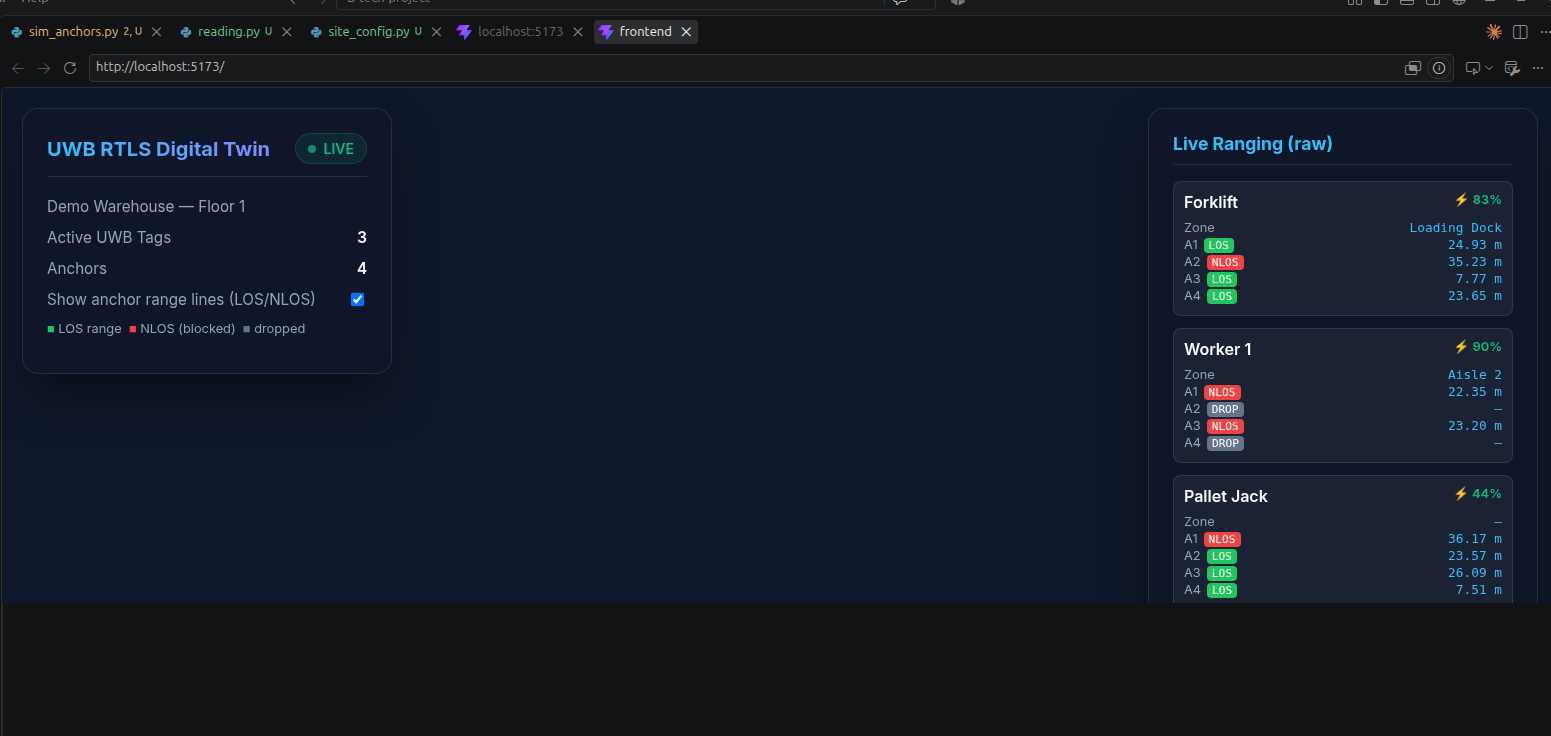
\includegraphics[width=\linewidth]{twin_screenshot.png}
      \begin{center}\tiny Live 3D digital twin\end{center}
    \end{column}
  \end{columns}
\end{frame}

\begin{frame}{Work Done --- Data-Driven NLOS Calibration (UTIL)}
  \begin{columns}[T]
    \begin{column}{0.5\textwidth}
      \begin{itemize}\small
        \item \texttt{calibrate\_from\_util.py} fits real range-error stats from UTIL
              ($\sigma_{\text{range}}=\sigma_{\text{tdoa}}/\sqrt{2}$) and patches \texttt{site.json}
              (\texttt{calibrated:UTIL-IJRR2024}).
        \item \textbf{Finding:} NLOS $\approx$ a \textbf{positive bias 0.03--0.40~m}, \emph{not} extra noise.
        \item Sim reads its model from config $\Rightarrow$ a \textbf{data change, not code change}.
      \end{itemize}
    \end{column}
    \begin{column}{0.5\textwidth}
      \small
      \begin{tabular}{lcc}
        \toprule
        Parameter & Before & After \\
        \midrule
        LOS noise $\sigma$ (m)   & 0.08 & \textbf{0.054} \\
        NLOS noise $\sigma$ (m)  & 0.30 & \textbf{0.054} \\
        NLOS bias min (m)        & 0.25 & \textbf{0.026} \\
        NLOS bias max (m)        & 1.20 & \textbf{0.399} \\
        \bottomrule
      \end{tabular}
    \end{column}
  \end{columns}
\end{frame}

\begin{frame}{Work Done --- UTIL Dataset Pipeline (real UWB data)}
  \begin{columns}[T]
    \begin{column}{0.5\textwidth}
      \begin{block}{What UTIL provides}
        \footnotesize
        \begin{itemize}\small
          \item Decawave \textbf{DWM1000}; 4 anchor constellations; $\approx$150~min of flights.
          \item Raw \textbf{TDOA}, SNR / power-difference (LOS/NLOS labels), IMU, altitude,
                \textbf{mm-accurate Vicon ground truth}.
        \end{itemize}
      \end{block}
      \begin{block}{Parsing \& alignment --- \texttt{dataset\_source.py}}
        \footnotesize
        \begin{itemize}\small
          \item Long-format event-log CSV; anchor geometry from the \texttt{survey-results} files.
          \item Pose column is \emph{not} synced to the TDOA row $\Rightarrow$ \textbf{interpolate truth}
                to each TDOA timestamp (1.2~m $\rightarrow$ $\approx$0.09~m error).
        \end{itemize}
      \end{block}
    \end{column}
    \begin{column}{0.5\textwidth}
      \begin{block}{Three uses of the data}
        \footnotesize
        \begin{enumerate}\small
          \item \textbf{Calibrate} the noise / NLOS model ($\sigma_{\text{range}}=\sigma_{\text{tdoa}}/\sqrt{2}$)
                $\rightarrow$ patches \texttt{site.json}.
          \item \textbf{Validate} the TDOA-EKF on real flights (0.18--0.33~m RMSE vs mm truth).
          \item \textbf{Train} a 2-component Gaussian mixture (EM) $\rightarrow$ \texttt{tdoa\_model.json}
                for the generative simulator.
        \end{enumerate}
      \end{block}
      \begin{block}{Honesty caveat}
        \footnotesize Cross-radio (DWM1000 $\neq$ DW3000): the fitted model is a \emph{prior needing
        DW3000 recalibration}, not a direct transplant.
      \end{block}
    \end{column}
  \end{columns}
\end{frame}

\begin{frame}{Work Done --- TDOA-EKF on Real Data + Generative Sim}
  \begin{itemize}
    \item \textbf{Walled-off TDOA-EKF} (off the delivery critical path) validated on real UTIL flights:
      \begin{itemize}\small
        \item \texttt{DatasetTdoaSource} replays a trial; truth \textbf{interpolated} to each TDOA timestamp
              (1.2~m $\rightarrow$ $\approx$0.09~m).
        \item \texttt{TdoaEKF}: 3D CV-EKF, $h(p)=\lVert p-a_B\rVert-\lVert p-a_A\rVert$ linearised each step;
              \textbf{chi-square gate} rejects NLOS outliers; Gauss--Newton cold start (no truth used).
      \end{itemize}
    \item \textbf{Generative TDOA simulator:} a learned 2-component Gaussian mixture (EM on UTIL residuals)
          drives \emph{any} editable layout via TDOA + EKF (\texttt{?map=wh-tdoa}).
  \end{itemize}
\end{frame}

\begin{frame}{Work Done --- Results}
  \begin{columns}[T]
    \begin{column}{0.46\textwidth}
      \scriptsize
      \begin{tabular}{p{3.4cm}c}
        \toprule
        Configuration & Error \\
        \midrule
        Range solver, sim LOS/NLOS        & $\approx$0.6--0.7~m raw \\
        + Constant-velocity Kalman        & $\approx$4--5\% mean $\uparrow$ \\
        TDOA-EKF, real UTIL const1/2      & \textbf{0.18--0.20~m} \\
        TDOA-EKF, real UTIL const3        & $\approx$0.33~m \\
        Generative TDOA sim (WH)          & $\approx$0.5~m horiz. \\
        \bottomrule
      \end{tabular}
      \vspace{6pt}

      \footnotesize\textbf{Takeaway:} bias dominates $\Rightarrow$ NLOS \textbf{weighting + calibration}
      matter more than a heavier filter.
    \end{column}
    \begin{column}{0.54\textwidth}
      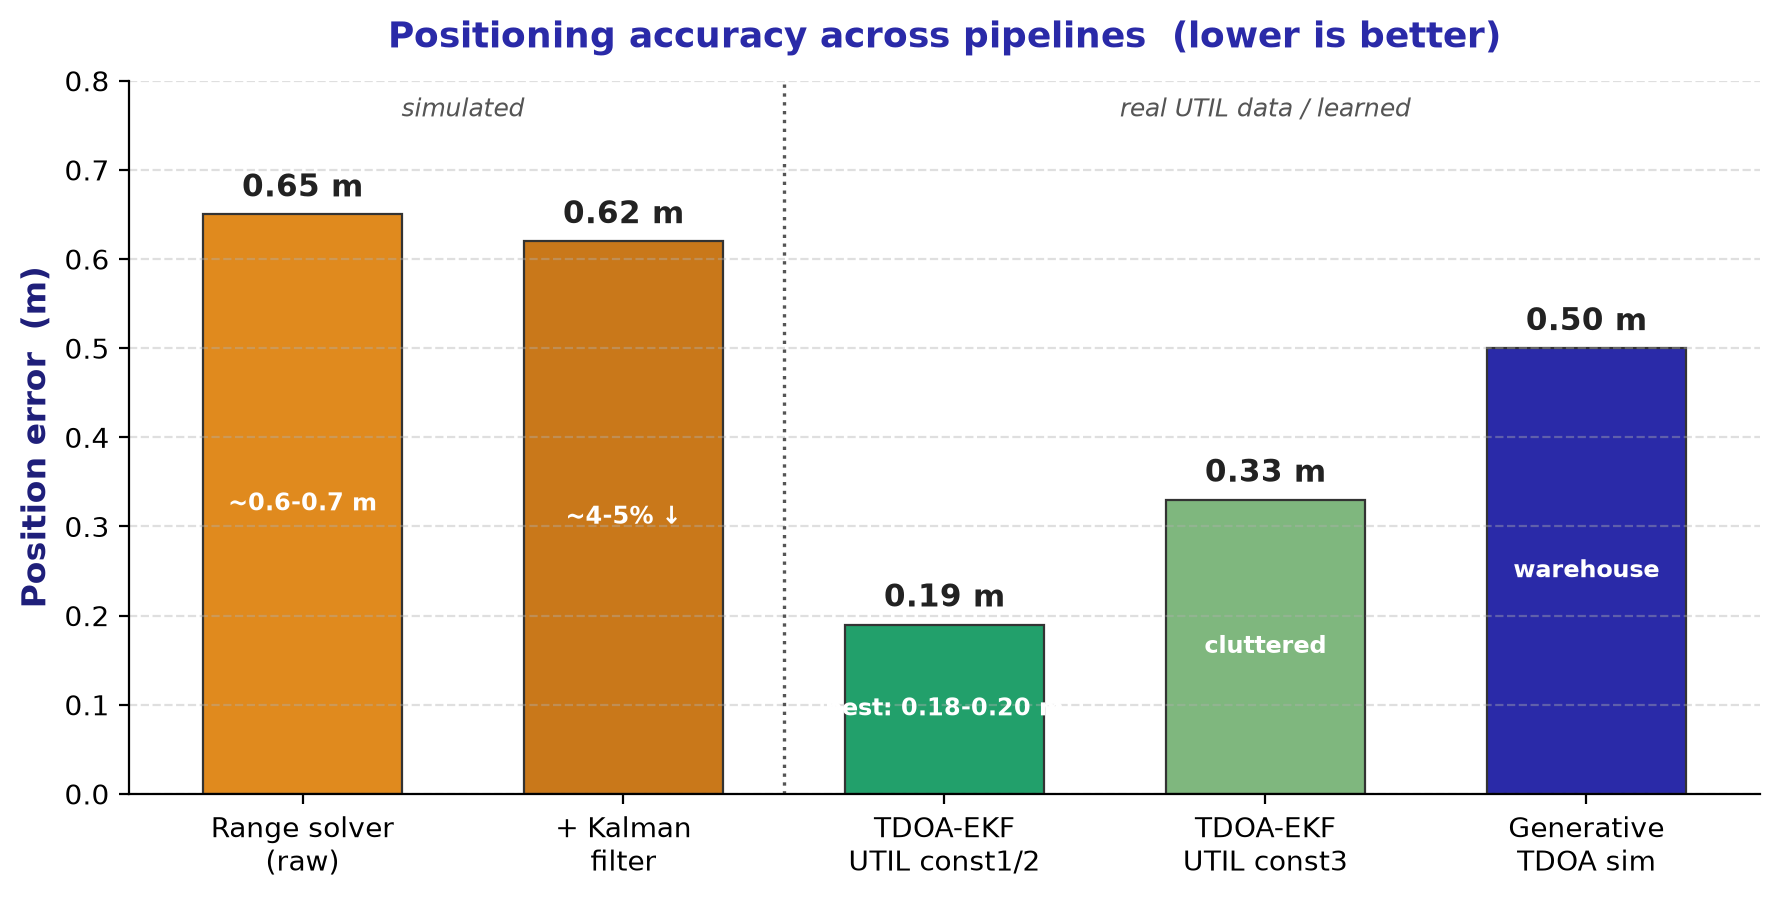
\includegraphics[width=\linewidth]{accuracy_chart.png}
    \end{column}
  \end{columns}
\end{frame}

\begin{frame}{Work Done --- Testing \& Status}
  \begin{columns}[T]
    \begin{column}{0.5\textwidth}
      \textbf{Verification}
      \begin{itemize}\small
        \item \textbf{21 automated tests (pytest), all passing.}
        \item Solver $<$1~cm on clean geometry; Kalman reduces mean error; calibration reproduces LOS $\sigma$ +
              positive-only NLOS bias; EKF on synthetic + real trials.
        \item \textbf{End-to-end demo:} raw fix jitters, Kalman track smooth, HUD shows filtered $<$ raw.
        \item \textbf{Hardware-readiness:} swapping \texttt{Sim}$\rightarrow$\texttt{Hardware} source is the \emph{only}
              change; engine untouched.
      \end{itemize}
    \end{column}
    \begin{column}{0.5\textwidth}
      \small
      \begin{tabular}{ll}
        \toprule
        Phase & Status \\
        \midrule
        1. Foundation \& framework   & \textbf{Done} \\
        3. Range multilateration     & \textbf{Done} \\
        4. Kalman filter fusion      & \textbf{Done} \\
        5. Digital-twin upgrades     & \textbf{Done} \\
        UTIL calibration             & \textbf{Done} \\
        TDOA-EKF (walled-off)        & \textbf{Built} \\
        Generative TDOA sim          & \textbf{Built} \\
        6. Basic AI (zones/predict)  & \emph{Pending} \\
        \bottomrule
      \end{tabular}
    \end{column}
  \end{columns}
\end{frame}

%==============================================================================
\section{Work Plan}
%==============================================================================
\begin{frame}{Work Plan}
  Remaining work and timeline:
  \begin{center}\small
  \begin{tabular}{p{6.5cm}l}
    \toprule
    Task & Timeline \\
    \midrule
    \textbf{Phase 6 --- Basic AI:} geofence / zone anomaly alerts + short-horizon
    trajectory prediction ($p + v\,\Delta t$ ghost marker) on the Kalman velocity & Phase 1 \\
    \textbf{Hardware bring-up:} implement \texttt{HardwareAnchorSource} for the real
    MaUWB\_DW3000 feed; re-tune noise/power on DW3000 & Phase 2 \\
    \textbf{In-situ validation:} collect tape-measured, NLOS-labelled DS-TWR traces to
    confirm the calibration transfer direction & Phase 3 \\
    \textbf{Anchor geometry:} add more / better-spread anchors to improve height
    observability and overall accuracy & Phase 4 \\
    \bottomrule
  \end{tabular}
  \end{center}
\end{frame}

%==============================================================================
\section{Publication and References}
%==============================================================================
\begin{frame}{Publication and References}
  \textbf{Publication}
  \begin{itemize}\small
    \item None yet. Target: a short paper on the \emph{data-driven NLOS calibration}
          result (``NLOS weighting calibrated on real UWB error reduced RMSE by X\%'').
  \end{itemize}
  \vspace{4pt}
  \textbf{References}
  \begin{thebibliography}{9}\footnotesize
    \bibitem{paszek} K. Paszek, D. Grzechca, A. Becker, ``Design of the UWB Positioning System Simulator for LOS/NLOS Environments,'' \emph{Sensors}, 21(14):4757, 2021.
    \bibitem{as2025} ``NLOS-Exclusion Based UWB Positioning Algorithm,'' \emph{Applied Sciences}, 15:02689, 2025.
    \bibitem{as2024} ``UWB Real-Time Location System Study,'' \emph{Applied Sciences}, 14:11005, 2024.
    \bibitem{util} W. Zhao, A. Goudar, X. Qiao, A. P. Schoellig, ``UTIL: An Ultra-wideband TDOA Indoor Localization Dataset,'' \emph{IJRR}, 2024.
    \bibitem{aej2018} ``UWB Indoor Localization Error Modelling,'' \emph{Alexandria Eng. J.}, 2018.
    \bibitem{makerfabs} Makerfabs, ``MaUWB\_DW3000 (ESP32 + DW3000, DS-TWR firmware),'' product docs.
  \end{thebibliography}
\end{frame}

{\setbeamertemplate{footline}{}
\begin{frame}[plain]
  \begin{center}
    {\Huge\color{structure}Thank You}\\[8pt]
    {\large Questions?}
  \end{center}
\end{frame}}

\end{document}
